%\section{Theory}
\section {Early Evidence of the Internal Structure of Nucleon}
\pdfcomment{magnetic moment of proton and neutron}
The first evident of nucleons being a composite particles comes form the 
measurement of their magnetic moment. For spin 1/2 elementary particles, the 
magnetic moment can be expressed as 
\begin{equation}
\mu = \frac{g}{2}\mu_B ~~~~ \mu_B = \frac{e\hbar}{2m},
\end{equation}
with $g$ expected to be $2$. Such measurement was first carried out by Otto 
Stern in 1933. And they found that the $g$ factor for proton is significantly 
greater than $2$. Since the neutron is a neutral particle, it was expected that
to have a zero magnetic moment. Stern and his team would later found that the 
neutron moment to be non-zero, suggesting that proton and neutron are composite
particles.
\pdfcomment{find appropriate citation. The original paper on proton magnetic
	moment is in Germany which I can't read}

In the 1950s, the proton form factor was measured using electron proton elastic
scattering experiments\cite{hofstadter1956}. The electron-proton elastic 
scattering in the laboratory frame can be expressed in the Rosenbluth formula
\begin{equation}
\dv{\sigma}{\Omega} = \frac{\alpha^2}{4E^2 \sin^2\left(\theta/2\right)} 
	\frac{E^\prime}{E} \left( \frac{G_E^2+\tau G_M^2}{1+\tau} \cos^2 
	\frac{\theta}{2} + 2\tau G_M^2 \sin^2 \frac{\theta}{2}\right)
	\label{eq:ep_cs},
\end{equation}
where $\tau$ is given by
\begin{equation}
\tau = \frac{Q^2}{4m_p^2}.
\end{equation}
And $E$, $E^\prime$ are the initial and final energy of the scattered electron.
The electric ($G_E\left(Q^2\right)$) and magnetic ($G_M\left(Q^2\right)$) form
factors are functions of the four momentum squared of the virtual photon. At 
low-$Q^2$ limit, these form factors can be interpreted as the Fourier transforms
of the charge and magnetic moment distribution of the nucleon. The deviation of
the neutron electric form factor from zero illustrate the existence of internal
structures in nucleons. Fig.\ \ref{fig:charge} shows the extracted proton and 
neutron charge density from the electric form factor taken from Ref.\ 
\cite{miller2007}.
\begin{figure}[htbp!]
    \centering
    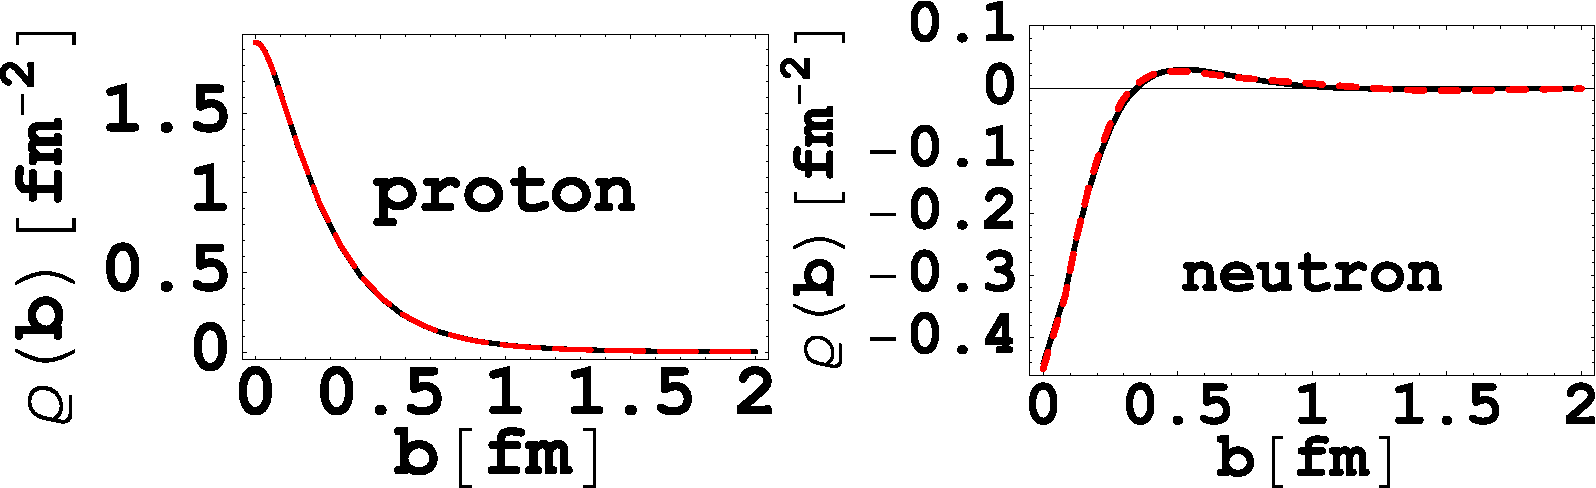
\includegraphics[width=0.9\linewidth]{./images/charge_distribution_rotated}
    \caption{The proton charge density (left panel) and neutron charge density
	(right panel). Taken from Ref.\ \cite{miller2007}}.
    \label{fig:charge}
\end{figure}


\section {Deep Inelastic Scattering}
\label{sec:dis}
Evidence of the point-like constituents in the nucleon first came from the deep
inelastic scattering (DIS) experiments \cite{breidenbach1969}, where a high 
energy lepton ($l$) is inelastically scattered of a nucleon ($N$), as 
illustrated in Fig.\ \ref{fig:DIS}
\begin{equation}
	l + N \rightarrow l^\prime + X.
\end{equation}
\begin{figure}[htbp!]
    \centering
    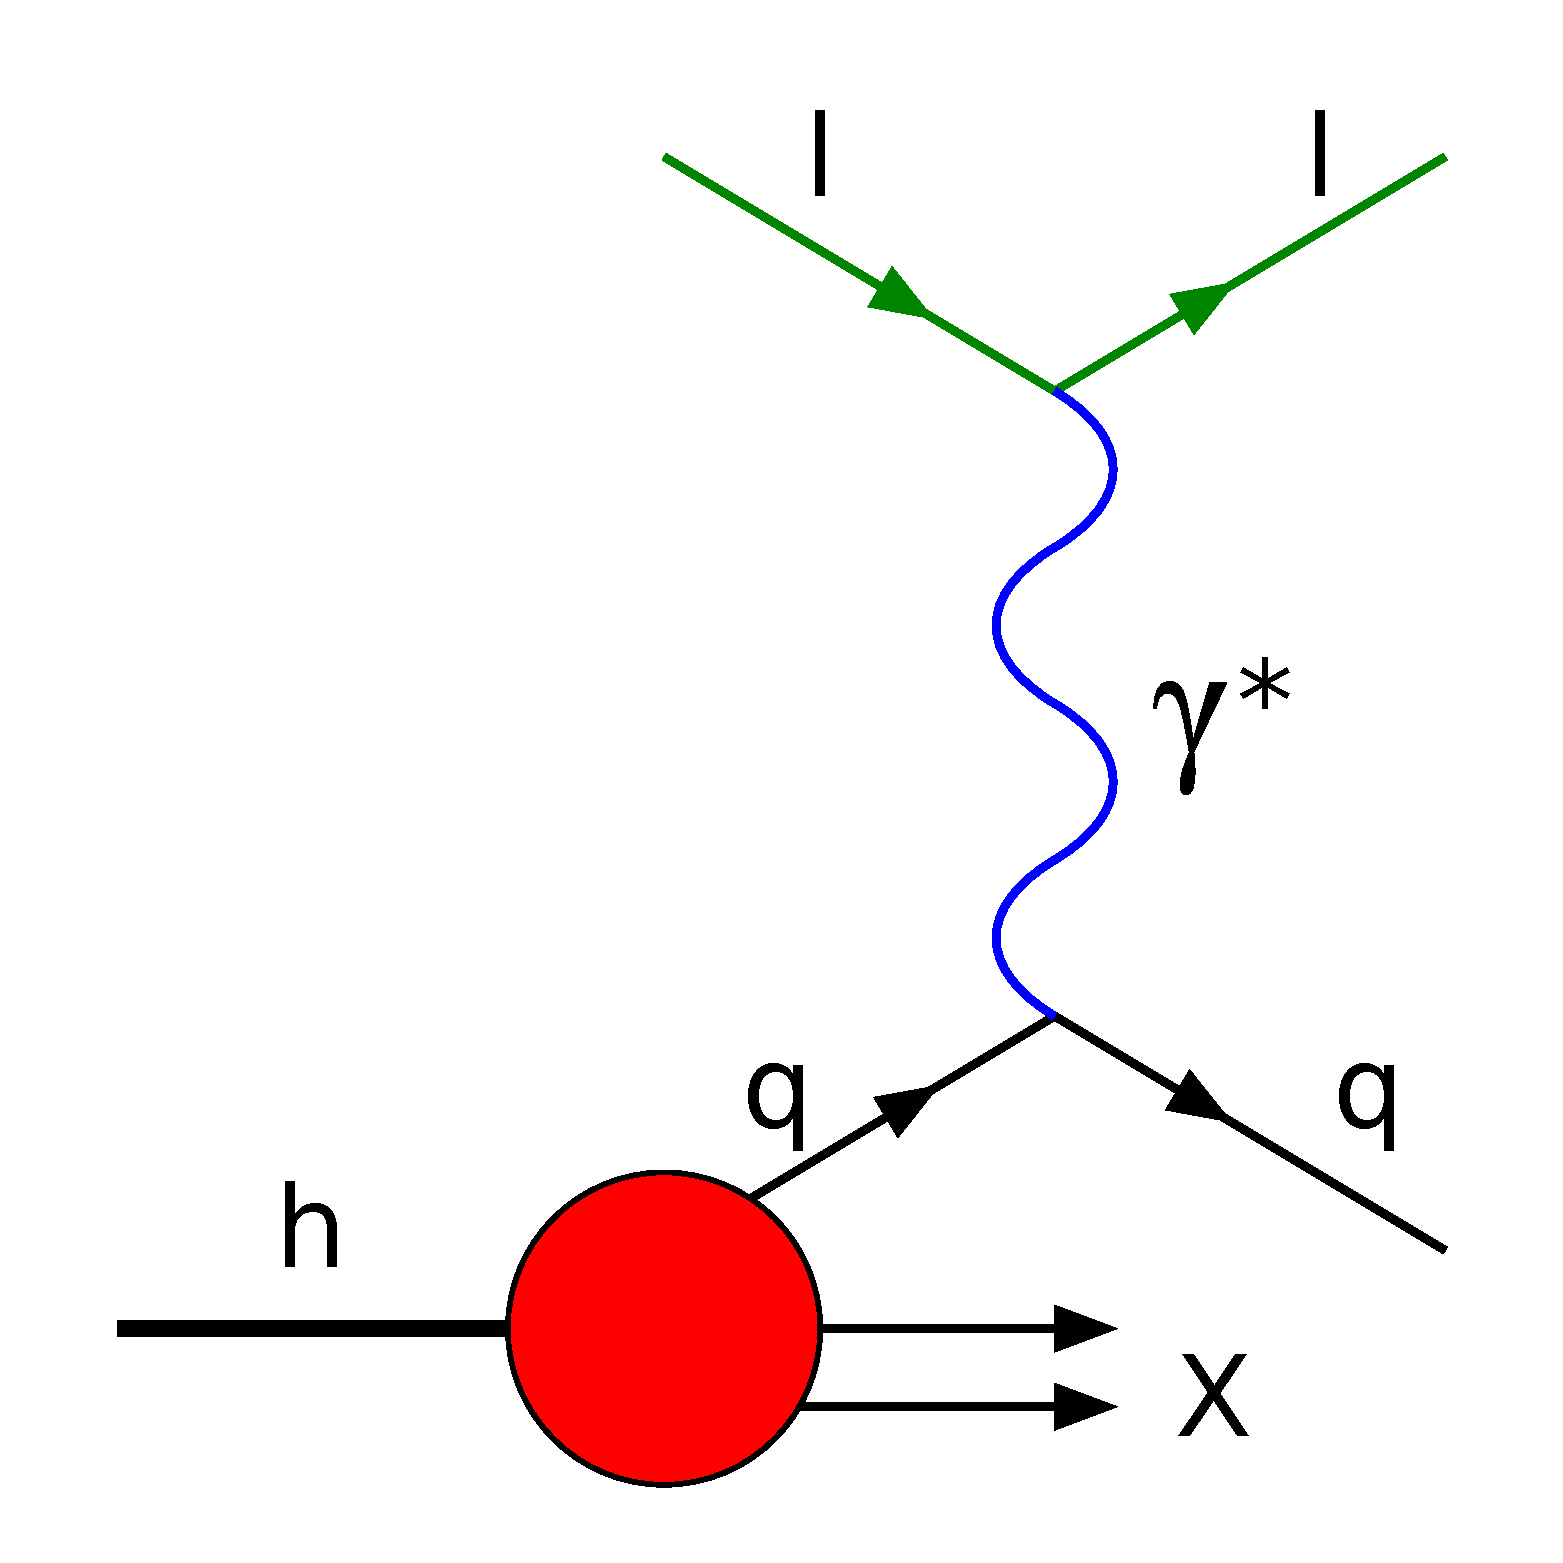
\includegraphics[width=0.5\linewidth]{./images/DIS}
    \caption{The Feynman diagram for DIS}
    \label{fig:DIS}
\end{figure}
Similar to Eq.\ \ref{eq:ep_cs}, the DIS cross section can be expressed as 
\begin{equation}
	\eval{\pdv{\sigma}{E^\prime}{\Omega}}_{DIS} = \frac{\alpha^2}{4E^2 \sin^4 
	\frac{\theta}{2}} \left[ W_2\left(\nu,Q^2\right)\cos^2
	\frac{\theta}{2} + W_1\left(\nu,Q^2\right)\sin^2 \frac{\theta}{2}
	\right],
	\label{eq:DIS_cs1}
\end{equation}
where $\nu$ is the energy transferred by the scattering lepton. It is also 
customary to the define the structure functions $F_{1,2}$ from $W_{1,2}$ as:
\begin{equation}
	\begin{split}
		F_1\left(x,Q^2\right) &= MW_1\left(\nu,Q^2\right),\\
		F_2\left(x,Q^2\right) &= \nu W_2\left(\nu,Q^2\right),
	\end{split}
\end{equation}
where $x=Q^2/2M\nu$ and $M$ is the mass of the nucleon. It was observed that 
these structure functions $F_{1,2}$ are independent of $Q^2$, as illustrated in
Fig.\ \ref{fig:w2}. Fig.\ \ref{fig:w2} shows the early measurements of the 
structure function $F_2=\nu W_2$ as a function of $Q^2$ for a fixed 
$x=1/\omega=0.25$ taken from Ref.\ \cite{friedman1972}. This observation is 
known as Bjorken scaling\cite{bjorken1969}.
\begin{figure}[htpb!]
	\centering
	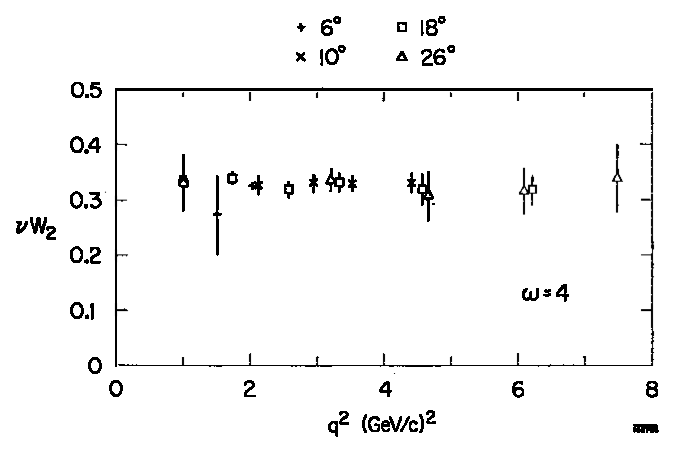
\includegraphics[width=0.5\linewidth]{images/nu_W2}
	\caption{Early measurement structure function $F_2=\nu W_2$ from 
	fixed-target electron–proton inelastic scattering at SLAC for 
	$x=1/\omega=0.25$ taken from Ref.\ \cite{friedman1972}. The observation 
	that $F_2(x,Q^2)$ is independent of $Q^2$ is known as Bjorken scaling. }
	\label{fig:w2}
\end{figure}

\section{Parton Model}
\label{sec:parton}
To explain the scaling behavior, Feynman proposed the parton model\cite{feynman1969}.
In this model,hadrons are treated as an extended objects which are made up of 
constituents (partons) held together by their mutual interaction. We now know 
these partons are quarks and gluons described by QCD, but this was not known at 
the time. Consider the DIS process, the hadron is Lorentz contracted in the 
direction of the collision in the center-of-mass frame, and the internal 
interaction are time dilated. Hence as the center-of-mass energy increases, the 
lifetime of the virtual partonic state is lengthened, and the time for the 
electron to pass trough the hadron is shortened. If the lifetime of the virtual
partonic states is longer than the duration of the electron-hadron interaction,
the partons are essentially frozen and the parton-parton interactions are 
neglectable. The hadrons can be considered as a collection of ``free'' partons,
and each parton may be thought of as carrying a definite fraction $x$ of the 
hadron's momentum. The high energy lepton in DIS can be treated as scattering 
of these partons elastically. The electron-parton elastic scattering can be 
calculated using perturbation QCD, where as the non-perturbation long-range 
interaction within the hadron is encapsulated in the Parton Distribution
Function (PDF) $f_{a/h}\left(x\right)$, which can be interpreted as the probability 
of finding a parton of species $a$ with fraction $x$ of the hadron's momentum. 
And the structure functions and the cross section can be written as a convolution
as non-perturbative PDF and the perturbative short range interaction. To Leading
order, the structure function $F_2\left(x\right)$ is given by
\begin{equation}
F_2\left(x\right)=x\sum_i e^2_i f_i\left(x\right),
\label{eq:F2_parton}
\end{equation}
where $e_i$ is the charge carried quark and antiquark of flavors $i$. Since, the 
gluon does not carry any charge, it does not enter the cross section at leading 
order. The ability to write the structure function and the cross section as a 
convolution of the non-perturbative PDF and pertubative short range interaction
is known as the factorization theorem \cite{collins1989}. These PDFs are also 
expected to be universal and independent of the details of the scattering 
process, as they describe the dynamics of the partons in a given hadron.

In the parton model, the structure functions $F_{1,2}$ are clearly related. And
from Eq.\ \ref{eq:DIS_cs1}, it is obvious that the structure function $F_1$ is 
related to the magnetic form factor $G_E$ in Eq.\ \ref{eq:ep_cs}. If the partons
are spin 0 particles, one would expect $F_1$ to be zero. In leading order of QCD,
only the quarks and antiquarks contribute to the cross section. Since quarks and 
antiquarks are spin 1/2 particles, this relation is given by the Callan-Gross 
relation\cite{callan1968,callan1969}
\begin{equation}
F_2\left(x\right) = 2x F_1\left(x\right).
\end{equation}
The measured deviation of the Callan-Gross relation, defined as 
\begin{equation}
K_0 = \frac{F_2}{2xF_1}-1,
\end{equation}
is shown in Fig.\ \ref{fig:callan_gross}, taken from Ref.\ \cite{kendall1991}. 
For large $Q^2$, $K_0$ is consistent with zero, establishing the parton spin as
1/2.
\begin{figure}
\centering
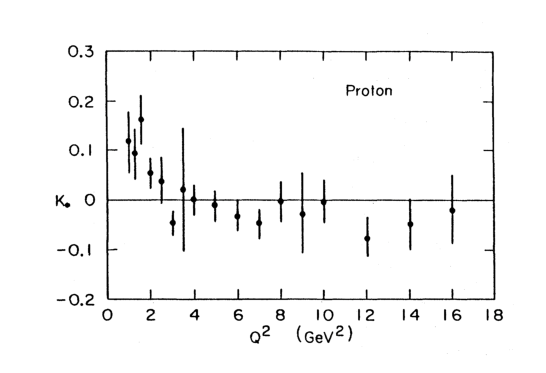
\includegraphics[width=0.5\linewidth]{images/Callan_Gross_relation}
\caption{The deviation from the Callan-Gross relation, defined as 
	$K_0=F_2/2xF_1 -1$, taken from Ref.\ \cite{kendall1991}. This result
	demonstrates the spin 1/2 nature of the partons.}
\label{fig:callan_gross}
\end{figure}

\subsection{Quantum Chromodynamics}
\label{sec:QCD}
\pdfcomment{QCD correction to parton model: Q2 dependence introduce by the 
	renormalization and factorization}
Quantum Chromodynamics(QCD) being a renormalizable theory, a regularization 
procedure and a set of renormalization prescription need to be specified. 
dependence

The renormalization scheme will also introduce a $Q^2$ dependency, known as scaling
violation. 

This $Q^2$ dependency can be understood as as due to the fact that a current with 
larger $Q^2$ probes a wider range of $k_\perp^2$ in the parton cloud of the target.

The QCD generalization of Eq.\ \ref{eq:F2_parton} is given by
\pdfcomment{check what nonsingulet means here}
\begin{equation}
F_2^{NS}\left(x,Q^2\right) = \int_0^1 \frac{\dd{y}}{y} \tilde{C}_2\left[\frac{x}{y},\frac{Q^2}{\mu^2},\frac{\mu^2_f}{\mu^2}.\alpha_s^{\mu^2}\right]\sum_i e_i^2 f_{i/p}(y,\mu_f,mu^2)
\end{equation}
As a consequence of the perturbative  calculation, a dependence on the renomalization
scale $\mu$ is introduced. The factorization scale $\mu_f$ is introduce to separate the 
low- and high-momentum regime, as the long-distance contributions cannot be calculated 
perturbatively and needs to be absorbed into the definition of the parton distribution
functions. It is also customary to choose $\mu_f^2=\mu^2$.

In leading-order of QCD, the coefficient function is given by
\begin{equation}
\tilde{C}_2 = \delta\left(1-\frac{x}{y}\right)+\frac{\alpha_s\left(Q^2\right)}{2\pi} \left[P_{qq}\left(\frac{x}{y}\right)\ln\frac{Q^2}{\mu}+R_2\left(\frac{x}{y}\right)\right]
\end{equation}
The splitting function $P_{qq}(z)$ is the Altarelli-Parisi kernel.\pdfcomment{citation}.
Since the leading logarithmic term is universal for all structure functions, it can 
be absorbed into a newly defined, $Q^2$ dependent parton distribution function:
\begin{equation}
f_{i/h}\left(x,Q^2\right) = f_{i/h}\left(x\right) + \frac{\alpha_s\left(Q^2\right)}{2\pi} 
	\int_0^1 \frac{\dd{\xi}}{\xi} f_{i/h}\left(\xi\right)\left[P_{qq}\ln\frac{Q^2}{\mu^2}\right]
\end{equation}

\subsection{Sum Rules}
\label{sec:sum_rules}
Since hadrons characterized by their quantum numbers, and these quantum numbers 
are carried by the constituent partons, these quantum numbers serve as constrains
on these PDF. For protons, there are two valance $u$ quarks and one valance $d$ 
quarks, hence
\begin{equation}
\begin{split}
	\int_{0}^{1} \dd{x} \left[f_{u/p} \left(x\right)-f_{\bar{u}/p} \left(x\right)\right]&=2,\\
	\int_{0}^{1} \dd{x} \left[f_{d/p} \left(x\right)-f_{\bar{d}/p} \left(x\right)\right]&=1,\\
	\int_{0}^{1} \dd{x} \left[f_{i/p} \left(x\right)-f_{\bar{i}/p} \left(x\right)\right]&=0 \qquad \text{other quark flavors}.
\end{split}
\end{equation}
And the momentum of the hadron should be distributed among the partons, hence
\begin{equation}
	\sum_{i=q,\bar{q},g}\int_{0}^{1} \dd{x} xf_{i/h}\left(x\right)=1.
\end{equation}
An important sum rule is the Gottfired sum rule\cite{gottfried1967}. It can be obtained
if we use the isospin symmetry to relate the neutron distributions to those of 
the proton, namely the (anti) up quark in the neutron would have the same distribution 
as (anti) down quark in proton, and vice-versa; the other quarks flavors and gluon
distribution would be the same in both proton and neutron. Using this relation
\begin{equation}
\begin{split}
	S_G & = \int_0^1 \frac{\dd{x}}{x}\left(F_2^{p} - F_{2}^{n}\right)\\
	    & = \frac{1}{3} \int_0^1 \dd{x} \left[u\left(x\right) - d\left(x\right) 
			+ \bar{u}\left(x\right) - \bar{s}\left(x\right)\right]\\
		& = \frac{1}{3} \int_0^1 \dd{x} \left[u\left(x\right) - \bar{u}\left(x\right)\right]
			- \frac{1}{3} \int_0^1 \dd{x} \left[d\left(x\right) - \bar{d}\left(x\right)\right]
			+ \frac{2}{3} \int_0^1 \dd{x} \left[\bar{u}\left(x\right)-\bar{d}\left(x\right)\right]\\
		& = \frac{1}{3} + \frac{2}{3} \int_0^1 \dd{x} \left[\bar{u}\left(x\right)-\bar{d}\left(x\right)\right]. 
\end{split}
\end{equation}
If one made the naive assumption that $\int_0^1\dd{x} \bar{u}\left(x\right)=\int_0^1\dd{x} \bar{d}\left(x\right)$,
then $S_G$ would be expected to be $1/3$. And this assumption can be tested using DIS.
One of the early measurements is from the New Muon Collaboration (NMC)\cite{amaudruz1991}. 
The measured $F_2^p-F_2^n$ by NMC is shown in Fig.\ \ref{fig:NMC_Gottfried}. 
\begin{figure}
	\centering
	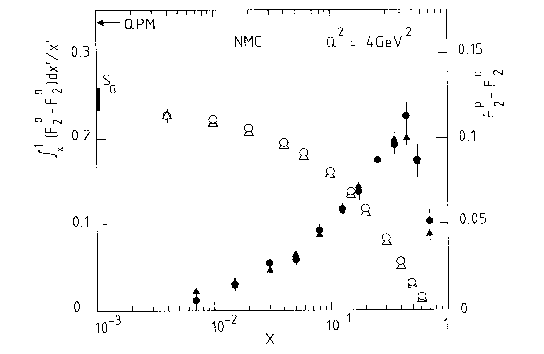
\includegraphics[width=0.7\linewidth]{images/Gottfried}
	\caption{The difference $F_2^p -F_2^n$ (solid and scale to the right) and 
		$\int_{x_{min}}^1 (F_2^p-F_2^n)\dd{x}/x$ (open and scale to the left) 
		determined by NMC, taken from Ref.\ \cite{amaudruz1991}. The extrpolation
		to $x_{min}=0$ is indicated by the bar.}
	\label{fig:NMC_Gottfried}
\end{figure}
The measured Gottfried sum to be $0.240 \pm 0.016$, which is significantly below 
$1/3$, suggesting the sea-quark asymmetry.


\section{Drell-Yan Process}
\label{sec:DY}
Another process for probing the hadron structure is the Drell-Yan process\cite{drell1970}.
As illustrated in Fig.\ \ref{fig:DY}, this process involves two partons from the 
two colliding hadrons to annihilate and form a lepton pair.
\begin{equation}
	h_A + h_B \rightarrow l + \bar{l} + X.
\end{equation}
\begin{figure}
	\centering
	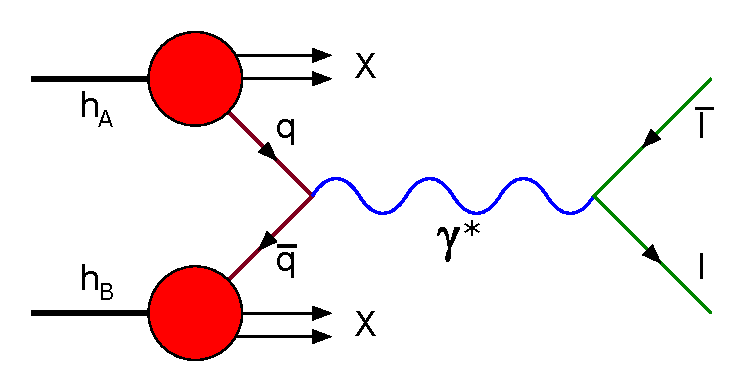
\includegraphics[width=0.7\linewidth]{images/Drell-Yan}
    \caption{The Feynman diagram for the Drell-Yan process}
    \label{fig:DY}
\end{figure}
Similar to DIS, the Drell-Yan cross section can be factorized into the non-perturbative
PDF and the purtabative parton-parton scattering. And the proof of factorization 
theorem for Drell-Yan can be found in Ref.\ \cite{collins1989}. At leading-order 
of QCD, the cross section can be written as
\begin{equation}
	\frac{d^2\sigma_{DY}}{dx_{1}dx_{2}} = \frac{4\pi\alpha^2}{9M^2}\sum_i e^2_i
		\left[f_{i/A}\left(x_1\right)f_{\bar{i}/B}\left(x_2\right) +
			f_{\bar{i}/A}\left(x_1\right)f_{i/B}\left(x_2\right)
		\right].
	\label{eq:DY_cs}
\end{equation}
Fig.\ \ref{fig:scaling} shows some of the existing data on DIS and Drell-Yan. By
performing a global fit to both DIS and Drell-Yan data, the parton distribution 
functions can be extracted. The ability to fit both DIS and Drell-Yan data using 
the same PDF demonstrate the universality of the PDF and the usefulness of the 
factorization theorem. 
\pdfcomment{factorization and universality of PDF, scaling plot for both DIS 
	and DY.May need better plot. Shows some PDF extraction}
\begin{figure}
	\centering
	\begin{subfigure}{0.45\linewidth}
		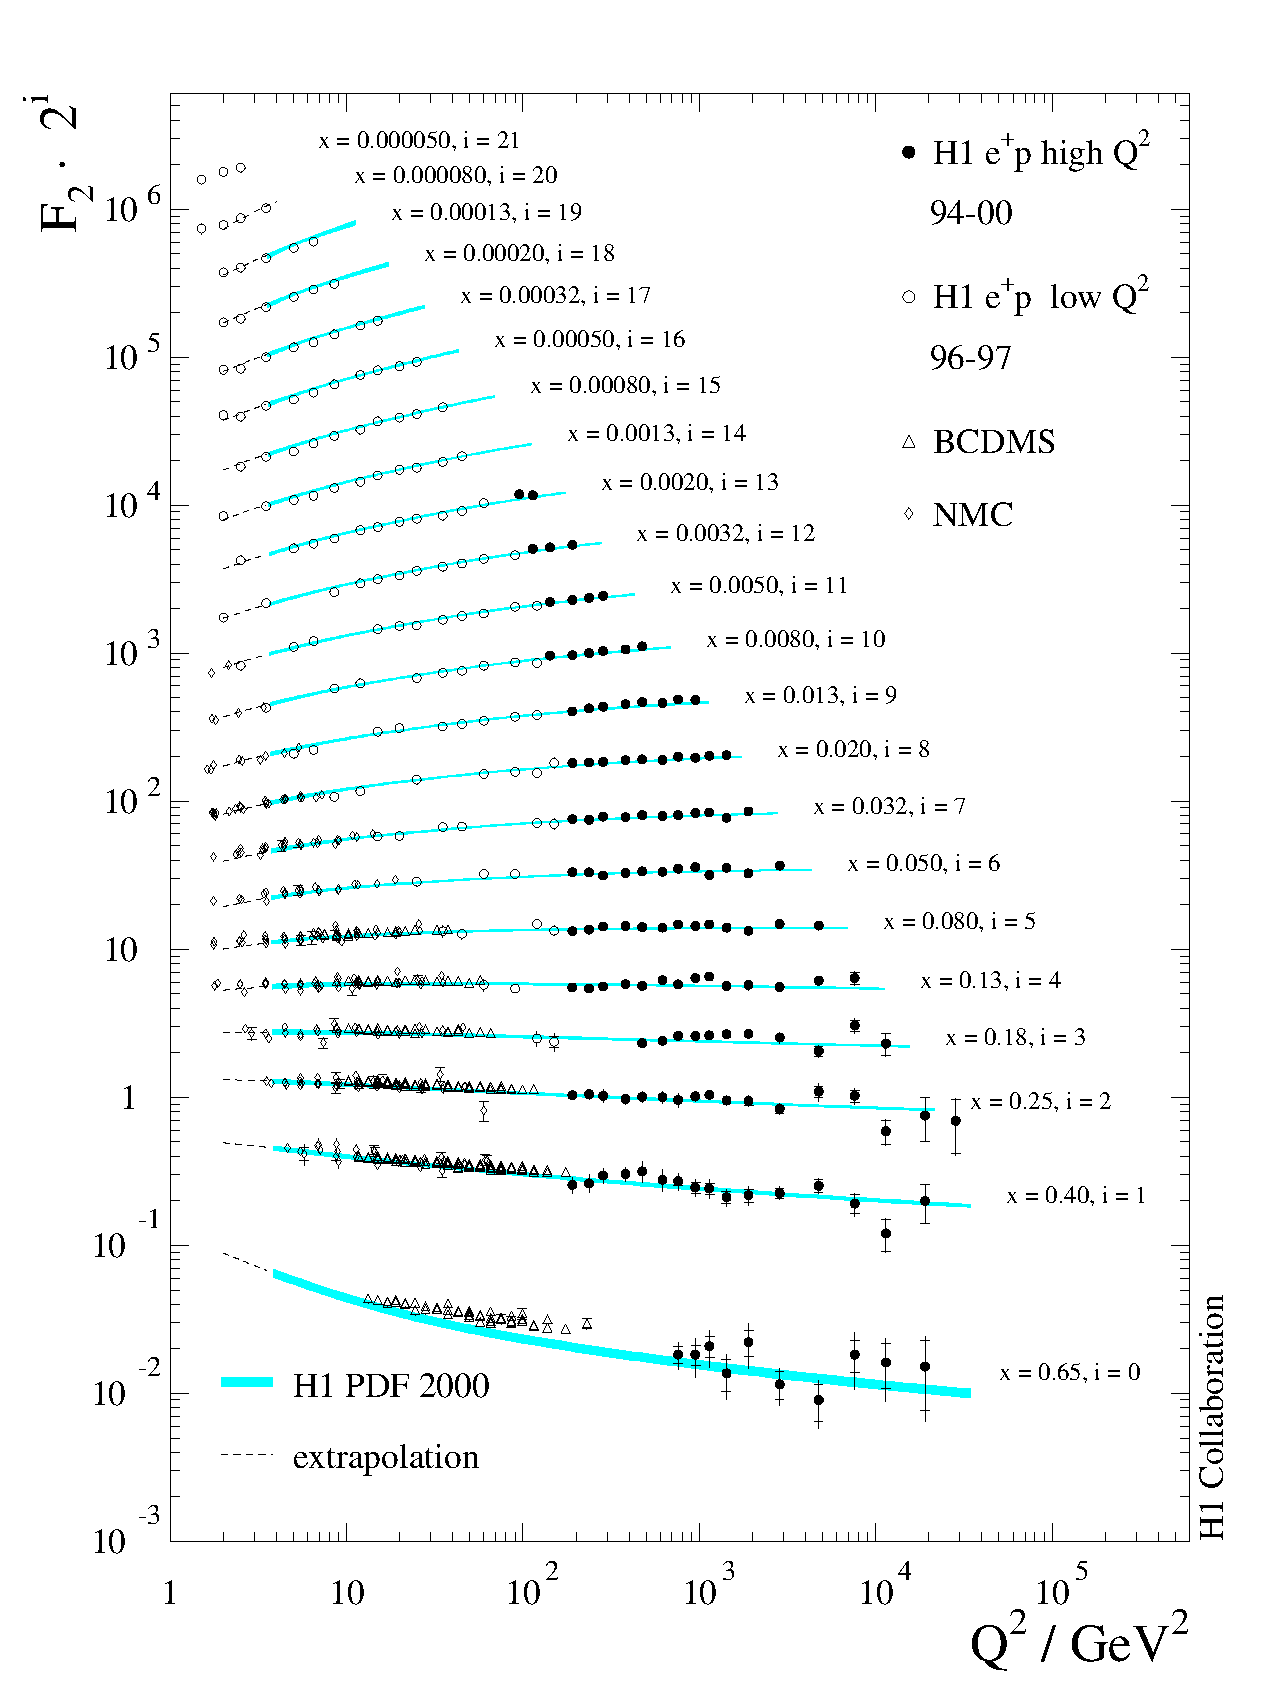
\includegraphics[width=\linewidth]{images/DIS_scaling}
		\caption{taken from Ref.\ \cite{theh1collaboration2003}}
		\label{subfig:DIS_scaling}
	\end{subfigure}
	\begin{subfigure}{0.45\linewidth}
		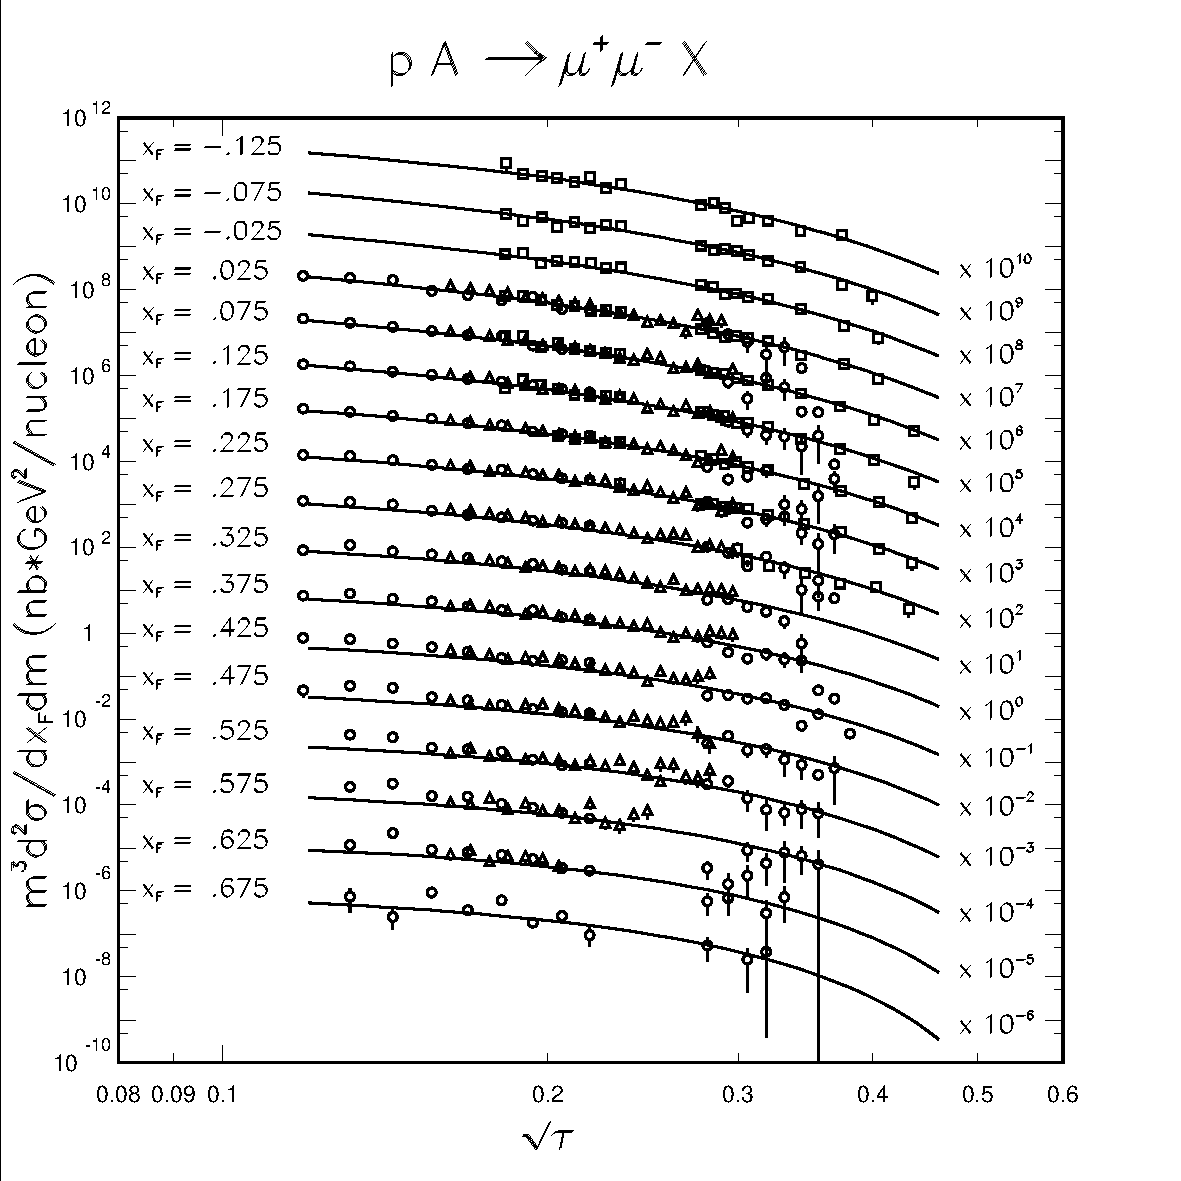
\includegraphics[width=\linewidth]{images/DY_scaling}
		\caption{taken from Ref.\ \cite{mcgaughey1999}}
		\label{subfig:DY_scaling}
	\end{subfigure}
	\caption{Compilation of data on DIS (\subref{subfig:DIS_scaling}) and 
		Drell-Yan (\subref{subfig:DY_scaling})}
	\label{fig:scaling}
\end{figure}
One of the advantages of Drell-Yan over DIS is the explicit separation of the quark
and anti-quark distributions in Eq.\ \ref{eq:DY_cs}. Since the structure functions
are dominated by valance quark distribution at large $x$, DIS is less sensitive to
the sea-quarks distribution at large $x$. On the other hand, in the high $x_F=x_1-x_2$
of Drell-Yan, the valance quark is more likely to come from the beam hadron, and 
the anti-quark is more likely to come from the target hadron. Hence, Drell-Yan can
be more sensitive to the anti-quark distribution than DIS. In particular, for high
$x_F$ and using the fact there are two up valance quarks in protons, the $(p+d/2(p+p))$
Drell-Yan cross section ratio can be approximated as 
\begin{equation}
	\frac{\sigma^{p+d}}{2\sigma^{p+p}} \approx \frac{1}{2} \left( 1+ \frac{\bar{d}\left(x_2\right)}{\bar{u}\left(x_2\right)} \right).
\end{equation}
Thus the Drell-Yan process has been used in many experiments to probe the sea-quarks 
asymmetry.


\subsection{E866/NuSea}
\label{sec:E866}
The E866/NuSea experiment was designed to measure the flavor structure of the sea 
quark over a broad range of $x$ to hiher precision than previous experiments. The 
experiment utilized the \SI{800}{\GeV} proton beam from the Tevatron on liquid 
hydrogen and deutrium targets. The deuterium over hydrogen cross section ratio 

\begin{figure}
	\centering
	\begin{subfigure}{0.45\linewidth}
		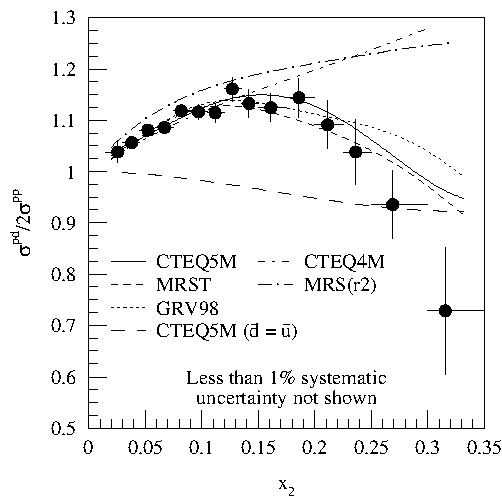
\includegraphics[width=\linewidth]{images/e866_csr}
		\caption{$(p+p)/2(p+d)$ Drell-Yan cross section ratio}
	\end{subfigure}
	\begin{subfigure}{0.45\linewidth}
		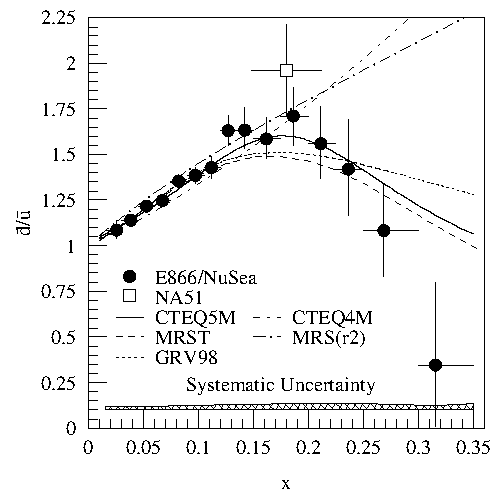
\includegraphics[width=\linewidth]{images/e866_dbarubar}
		\caption{$\bar{d}/\bar{u}$ extracted from E866 result.}
	\end{subfigure}
	\caption{The E866 result taken from Ref.\ \cite{fnale866/nuseacollaboration2001}}
\end{figure}



\section{Charmonium Production}
\label{sec:jpsi}
The mechanism for charmonium production can be separated into two parts, the 
production of heavy-quark pairs and the subsequent hadronization into 
quarkonium states. One of the early approaches is the Color Evaporation method 
(CEM)\cite{einhorn1975,bodwin1995,bodwin1997}. The heavy-quark pairs production
is expanded in terms of the strong coupling constant s and is calculated with 
perturbative QCD (pQCD). CEM then assumes a constant probability $F$ for the 
$c\bar{c}$ pairs to hadronize into different charmonium state and this 
probability is independent of the kinematics or the production subprocess. The 
charmonium production cross section in the CEM framework can be expressed as
\begin{equation}
\eval{\dv{\sigma}{x_{F}}}_{J/\psi\left(\psi^\prime\right)} =
	F_{J/\psi\left(\psi^\prime\right)} \sum_{i,j=q,\bar{q},g} \int_{2m_c}^{2m_D}
\end{equation}


\pdfcomment{CEM and NRCD}

\pdfcomment{what is physical significant of the nuclear dependence}

